\section{Inserting Edges}
\label{sect:inserting-edges}

As clusters in our data set grow increasingly similar, we may want to indicate this similarity with a new edge between two clusters in the cluster graph. However, because the cluster graph is internally triangulated, we cannot insert any more edges on the inside of the graph. We can only insert edges in the outer face. Inserting an edge in the outer face is also only possible if it preserves the internal triangulatedness of the cluster graph. Inserting an edge $\{u,w\}$ in the outer face is therefore only permitted if $u$ and $w$ have a neighbor $v$ in common such that adding the edge forms a new triangular face with $v$. A valid edge insertion is illustrated in \cref{fig:insert-edge-outside-example}.

\textbf{Insert edge on outer face:} Edges between nonadjacent vertices $u, v$ on the outer face may only be inserted if they preserve the graph's internal triangulatedness, \ie{} they don't create holes in the graph. Adding such an edge creates a new internal face and is therefore only possible iff $u$ and $v$ have a neighbor in common.

\begin{figure}[H]
	\centering
	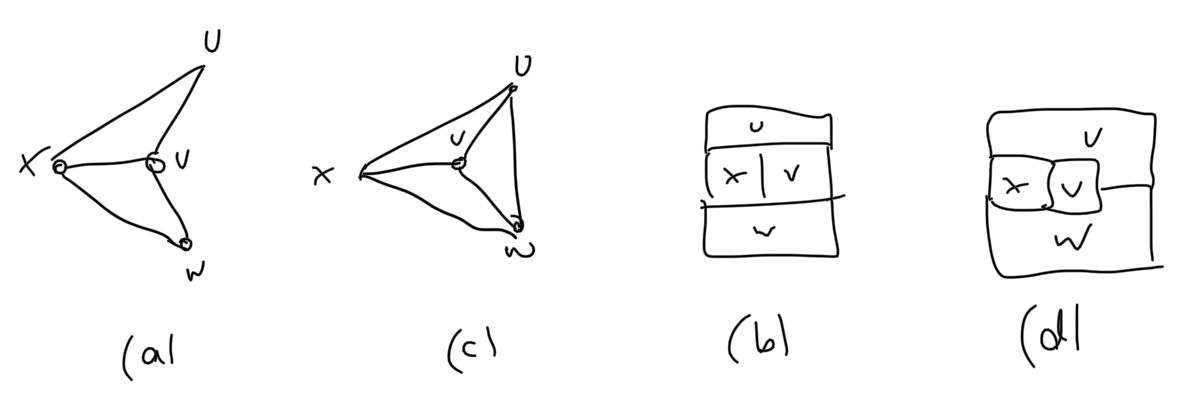
\includegraphics[height=30mm]{Resources/InsertEdgeOutside.png}
	\caption{A cluster graph and a polygonal dual thereof, before (a, b) and after (c, d) inserting the edge $\{u,w\}$ to form a triangular face with $v$.}
	\label{fig:insert-edge-outside-example}
\end{figure}
